\subsection{Network Architecture}

Our proposed network architecture (\autoref{fig:network}) consists of a basic 3D-UNet as implemented for the first time by \citeauthor{ronneberger_u-net_2015-1}~\cite{ronneberger_u-net_2015-1}.
It is composed of an encoding and a decoding part connected by skip-connections.
The encoding part is used to analyse the given input and transform it into a more abstract presentation level. 
This is achieved by consecutive application of 3D convolutions to the input.
Decoding translates this higher level of representation to the interpretable 3D space by applying 3D transposed convolutions.
Skip connections are utilized to incorparate a lower level of presentation into decoding part and preserve details from the input masks.\\
We adapted the downsampling depth of the proposed network due to memory limitations when using 3D data to a factor of 8. 
Maximum layer depth was 512 in the bottleneck connection. 
Skip connections were used before each pooling layer. 
To include a multitude of information from the patient as well as the \acs{RT} plan, we used five input volumes as proposed by \citeauthor{kontaxis_deepdose_2020}~\cite{kontaxis_deepdose_2020} concatenated along the forth dimension, resulting in an input volume of size $5 \times width \ (W) \times height \ (H) \times depth \ (D)$.
Resolution for all input volumes were set to the resolution of our CT scans with voxel dimensions of $1.1718 \times 1.1718 \times 3$ mm\textsuperscript{3} in the coronal, sagital, and tansversal plane. 


\begin{figure}[!b]
    \centering
    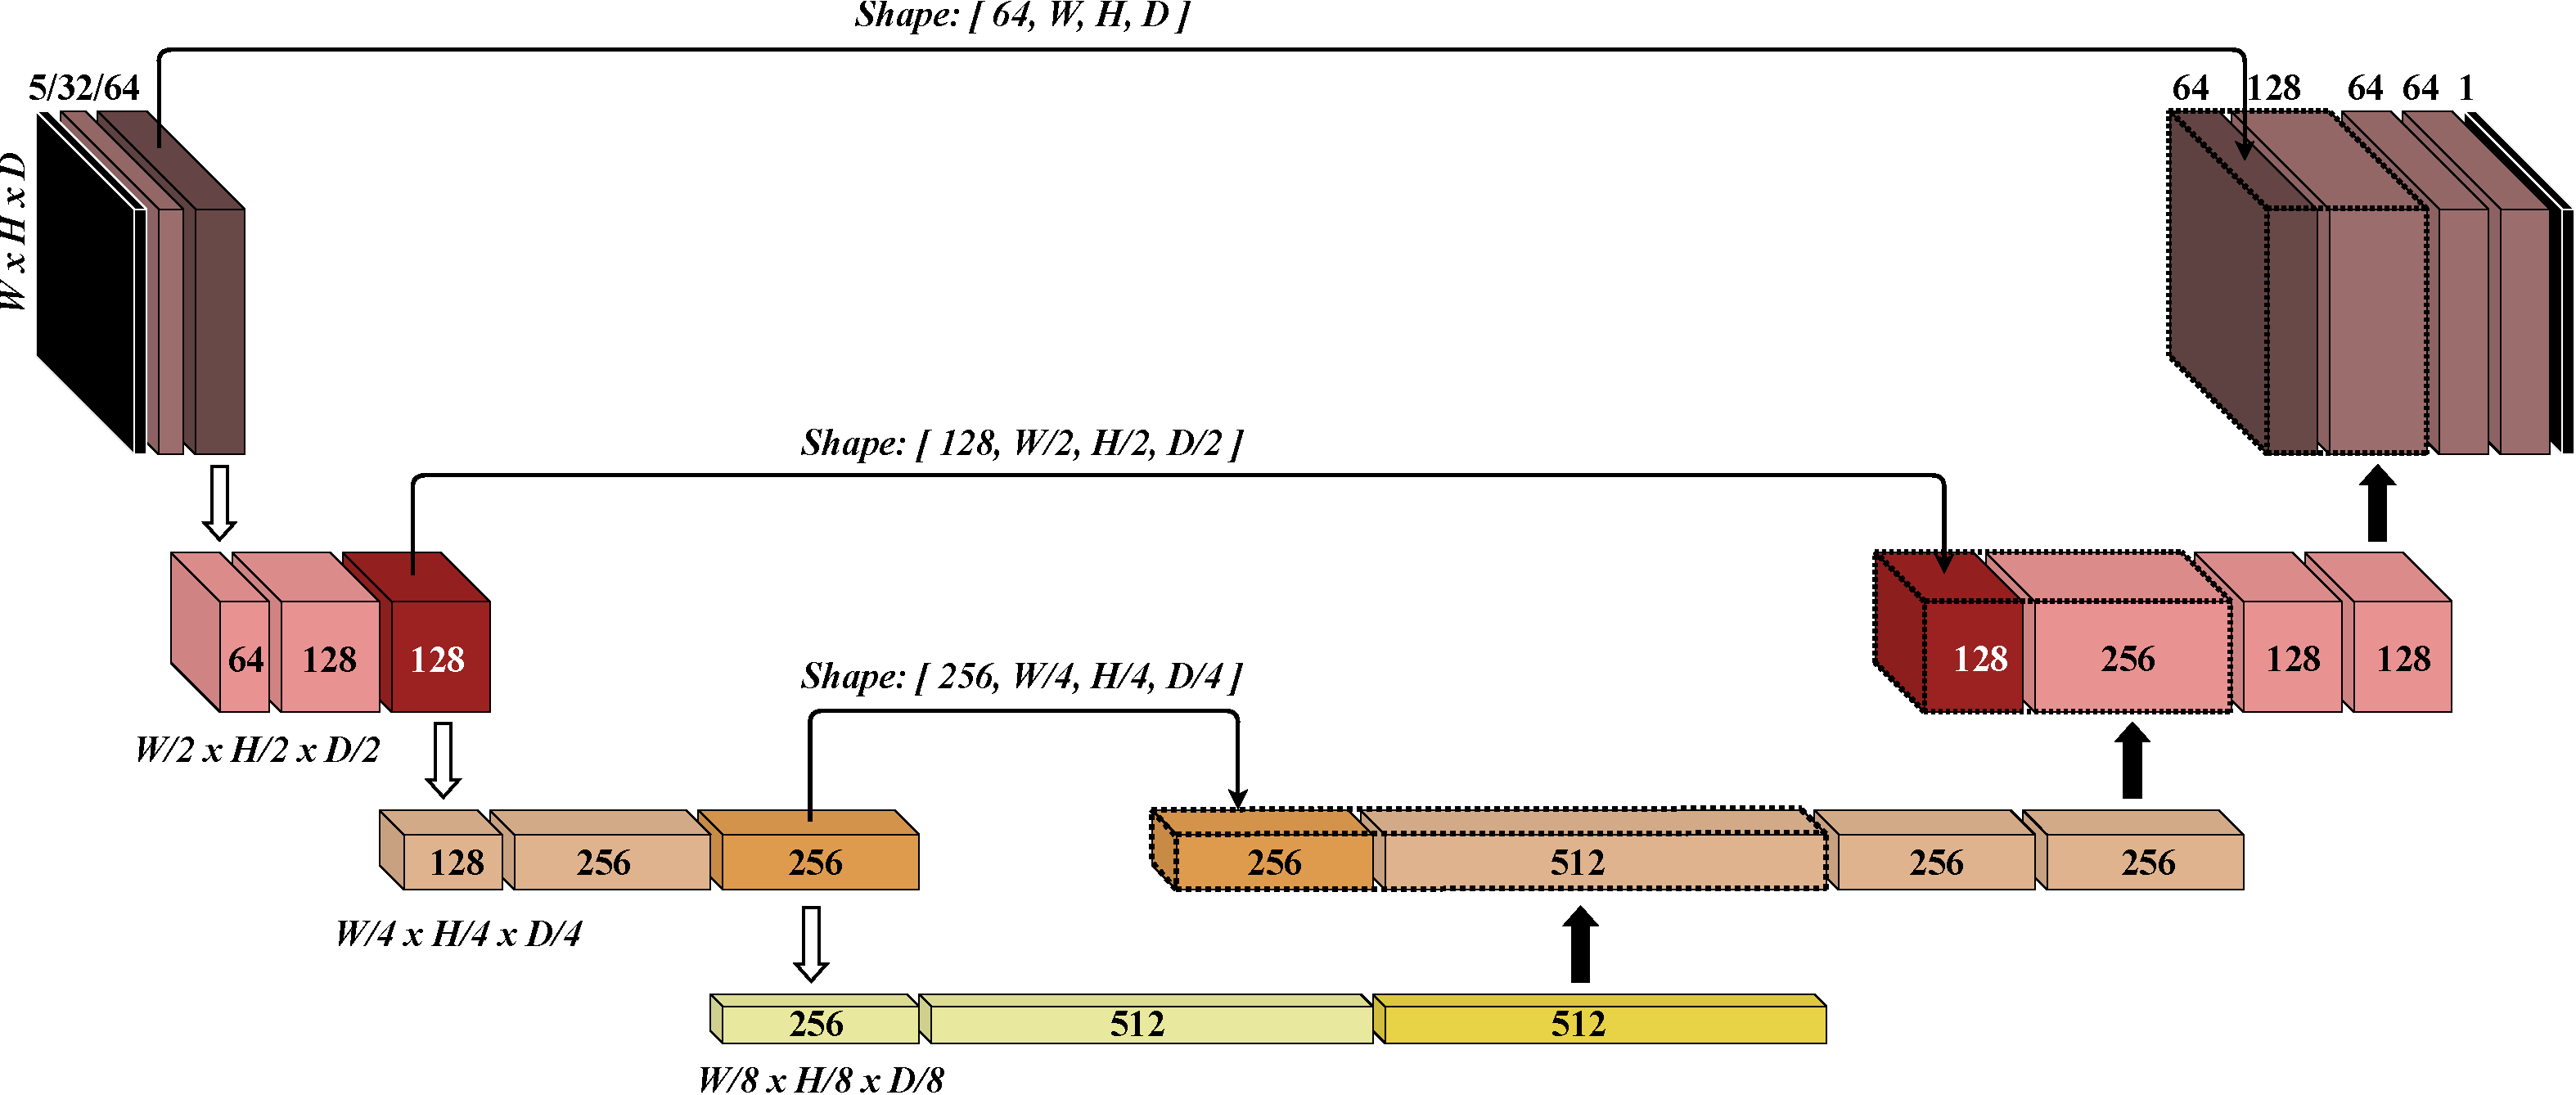
\includegraphics[width=0.9\textwidth]{UNET.pdf}
    \caption{Basic scheme of adapted network architecture with a downsampling ratio of 8 and a maximum depth of 512 in the bottleneck layer. Input dimensions: $5 \times W \times H \times D$; Output dimensions: $1 \times W \times H \times D$}\label{fig:network}
\end{figure}

\subsection{Network Input \& Output}

\subsubsection{Network Input}

The network expects five 3D volumes concatenated along their fourth dimension resulting in a 4D input. 
These five 3D volumes (\autoref{fig:masks}) combine different spatial, anatomical as well as accelorator information into the training data. 
By doing so gantry as well as accelerator head information can be directly translated into 3D space, which makes them interpretable for the network. 

\setlength{\hangingindent}{1em}

\begin{hangingpar}
    \item \textbf{(a) Beam Shape}: The trajectory of the beamshape into 3D space is of crucial importance. 
    Combining information from \acs{MLC} configurations as well as gantry angle provides the network with crucial information about the translation of the beams eye view into 3D space. 
    Information about which voxel is intersected or partially intersected by the beam is stored in this mask. 
    To additionally account for the output factor, the fieldsize of each segment is stored in each voxel intersected with the beam field. 
    Voxel values of partially clipped voxels are scaled down by the percentage of the voxel that lies within the field. 
    The output factor describes the physical process of increasing photon scatter into the central beamline for increasing fieldsizes. 
    
\end{hangingpar}

\begin{hangingpar}
    \item \textbf{(b) Center Beam Line Distance}: 
    Flattening filters are used to create uniform field distribution for photon beams from conventional accelerators.
    Flattening filters are not built into MR-Linac which makes it \ac{FFF}. 
    Beamprofiles of the MR-Linac are therefore not uniform.
    The dose profile peaks in the central beam line from where it flattens out to the edges of the field.
    Therefore, fields that are distant from the central beamline induce slightly lower doses than fields in the direct center.
    Each voxel in this mask is therefore assigned to its minimum distance from the central beamline. 
\end{hangingpar}

\begin{hangingpar}
    \item \textbf{(c) Source Distance}: 
    The radiation pattern of photons from the accelerator head can be assumed to be the front of a spherical wave. 
    The photon fluence is therefore decreasing with the square of the distance from the source. 
    The source distance mask takes this physical relationship into account. 
    Each voxel within the volume is assigned its distance to the source, taking into account the different voxel dimensions in the different spatial directions. 
    
\end{hangingpar}

\begin{hangingpar}
    \item \textbf{(d) CT}: 
    Dose deposition and interactions of particles depend on their energy as well as the electron density of the affected volume. 
    As the initial energy of the radiated photons is assumed constant, the impact of the electron density of the volume (in this case the patients anatomy) is responsible for the different interaction processes of photons as well as secondary electrons. 
    \ac{HU} of the patient's anatomy acquired from a \ac{CT} scan are stored in each voxel of the volume. 
    Photons radiated from gantry angles below the treatment couch interact partly inside it, therefore it was included in the \acs{CT} mask. 
\end{hangingpar}

\begin{hangingpar}\label{par:radiological_depth}
    \item \textbf{(e) Radiological Depth}: 
    A photon beam that passes through the interaction medium loses energy on its path. 
    Therefore, the path that a particle follows through a medium is highly relevant for the \acs{DD} effects. 
    Combining the information of the source distance of each voxel in combination with the density of the patients anatomy results in the radiological depth.
    It is calculated by the summation of the partial path of a casted ray through each intersected voxel in the medium multiplied by the \acs{HU} value of each respective voxel.
    Information about the density of prior tissues is given in each voxel value.
    Consequently the same spatial depth in a dense material results in a higher radiological depth than the same depth in soft tissue.
\end{hangingpar}

Particles interact negligibly in air, therefore all masks were set to zero where the CT masks was 150 \acs{HU} over the value of air. Air or low density volumes inside the body of the patient were not affected by this step to account for the \acs{ERE} on the surface of air cavities inside the patient. 

\begin{figure}
    \centering
    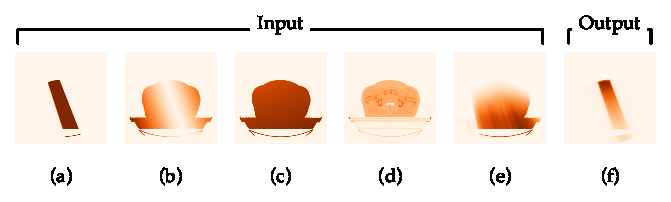
\includegraphics[width=\textwidth]{masks.pdf}
    \caption{Examplary input and output for a single segment of a prostate plan. (a): beam shape, (b): center beam line distance, (c): source distance, (d): CT, (e): radiological depth, (f): dose distribution, }\label{fig:masks}
\end{figure}

\subsubsection{Network Output}

The network combines the information from the five 3D volumes and yields a single volume with the respective dose distribution. 
Spatial dimensions for width, height and depth as well as voxel dimensions are preserved during inference. 
A respective dose distribution (f) for the input ((a)~-~(e)) from a segment taken from a prostate cancer treatment plan is depicted in \autoref{fig:masks}.

\subsection{Training Data Generation}

All training data was generated from patient data taken from the institutional database of radiotherapy treatment plans. 
Information for all input masks are given in the CT scan, the dose file as well as the plan file. 
The patients anatomy for the CT masks is taken from the CT files and adjusted to the right slice thickness, due to different aquisition protocols using 2~mm or 3~mm slice spacing. 
Dose distribution used as training target for each segment were calculated using the EGSnrc open source software package provided under~\cite{noauthor_nrc-cnrcegsnrc_2021}. 
The work of \citeauthor{friedel_development_2019}~\cite{friedel_development_2019} enabled us to accurately simulate single segment dose distributions for the MR-Linac. 
Simulation of all segments was done using a remote \ac{HPC} solution provided by the state of Baden-Württemberg. 
Coordinate system orientation of the patient's anatomy as well as \ac{MLC} and gantry positions are given in the dose and plan file. 
Simulation of $10^7$ particles took around 4 hours on average.
The 3D input volumes to the network were calculated using in-house developed python scripts with the provided information from CT, dose and plan files. 
The central beam line distance and source distance were calculated using the isocenter information from the DICOM-plan file and the respective coordinate system provided from the CT-DICOM files.
The CT mask was directly taken from the CT images and resized to fit the spatial resolution. 
Ray tracing was used to calculate the radiological depth mask with information from the CT and the gantry position which was taken from the DICOM-plan file.
Information about each segments \acs{MLC} configuration and gantry angle were used to project the beams eye view into 3D space for the beam shape mask.

\subsection{Network Training}

Four Nvidia GTX 2080 Ti, provided by the cloud of the Tübingen Machine Learning Cluster of Excellence, were used to increase the \acs{GPU} memory to 44 GB.
This enabled a batchsize of 128 with a patch size of $32 \times 32 \times 32$ voxels resulting in a spatial field of view of $37.5 \times 37.5 \times 96$~mm\textsuperscript{3}. 
After every epoch, the model performance was assessed on the validation set and the top 5 models were saved. 
The ADAM optimizer was used with 0.9, 0.99, $10^{-8}$ for $\beta_1$, $\beta_1$ and $\epsilon$ respectively. 
An initial learning rate of $10^{-4}$ was used. If the validation loss did not decrease or the gamma passrate on the valdiation set did not increase over 50 epochs the learning rate was decreased by a factor of 10. 
When a learning rate of $10^{-6}$ was reached and no performance increase was noted over 50 epochs the training was stopped to prevent overfitting and to save computational resources.
 

\subsubsection{Dataloading}

Memory usage is a serious concern in the application of deep learning and espeacially when dealing with 3D data sets. 
In our case not only the memory usage in the \ac{GPU} but also in the \ac{RAM} is of importance. 
In conventional applications the network training is divided into epochs, where the network sees every single instance before validation.
The present training data is therefore loaded into the \acs{RAM} and can be quickly accessed from there to pass it onto the \acs{GPU} memory.
Our here posed problem of dose deposition prediction is a 3D problem with input volumes of multiple hundreds of megabytes per input segment.
Loading all data into the \acs{RAM} was therefore not applicable. 
A solution to this problem is to load individual segments on the fly into the RAM and then process it.
This solution was not applicable for us because loading times were long compared to processing the segment during training, which would significantly slow down training.
We therefore developed a partial on the fly dataloading inspired by the \emph{Queue} class from \citeauthor{perez-garcia_torchio_2021}~\cite{perez-garcia_torchio_2021} open source python libary \emph{TorchIO}.
Classical augmentations in the form of shearing, warping or zooming were not applicable in our case because of the trivial relations between the augmentation and the \acs{DD}.
To still achieve additional variation in training data we employed patch based training. 
With this approach a multitude of patches can be extracted from the same segment volume, increasing the variety in training data.
To combine the semi-on-the-fly dataloading and the patch based training, multiple volumes are loaded into the RAM and then processed together as depicted in \autoref{fig:dataloading}. 
A fixed amount of training data is loaded from the randomized training data pool into the \acs{RAM}. 
From this set of training volumes a subset of patches from each volume is extracted and stored in a queue of patches, which is then shuffled and batch-wise passed onto the \acs{GPU} and the network. 

\begin{figure}
    \centering
    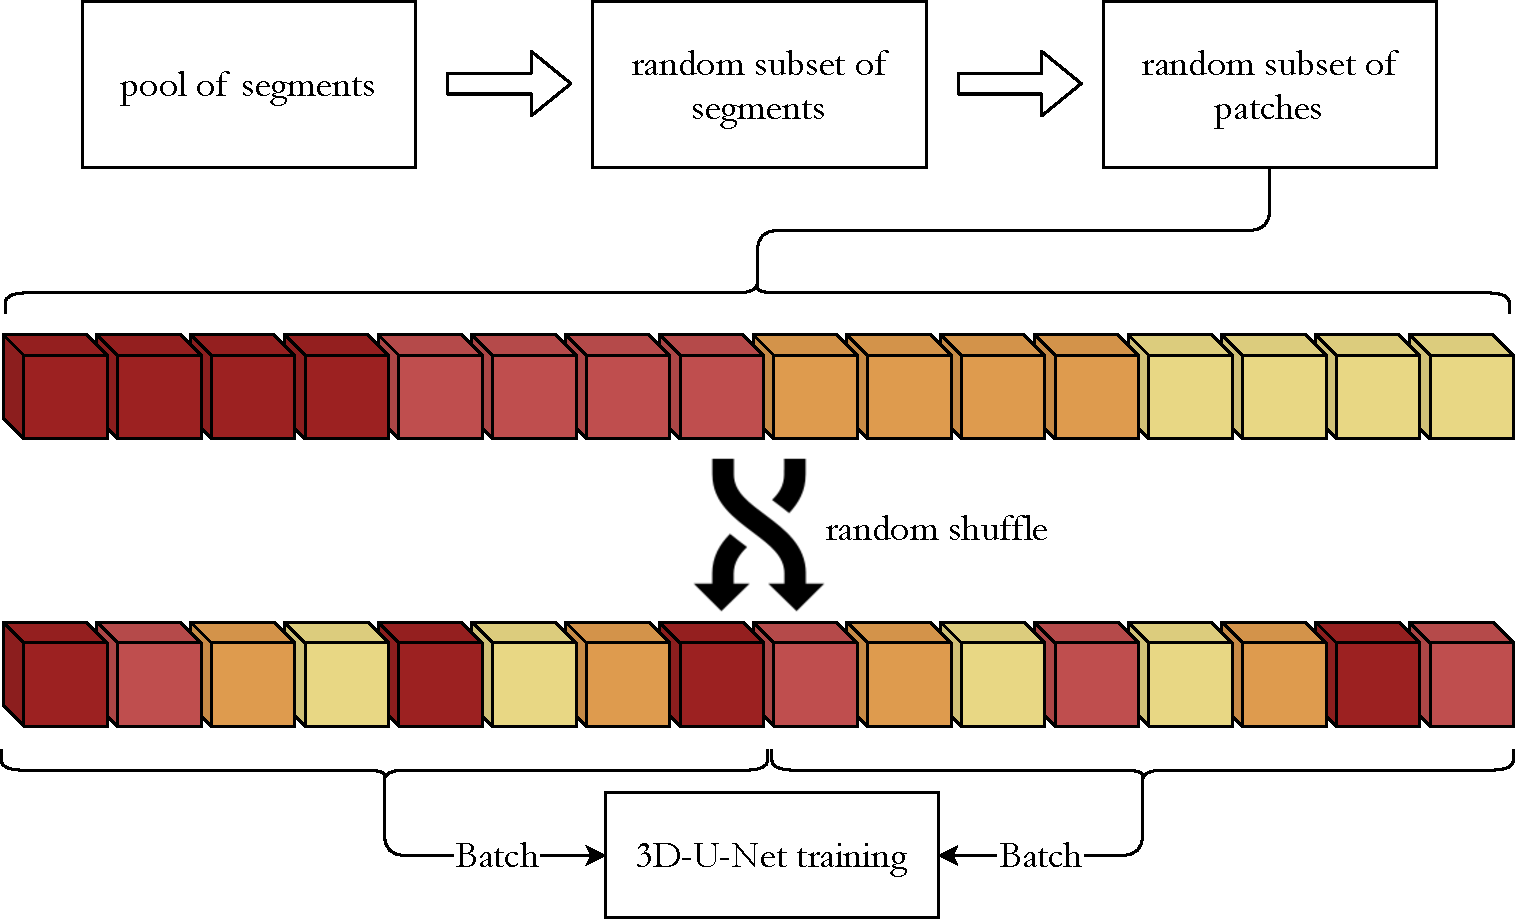
\includegraphics[width=0.7\textwidth]{dataloading.pdf}
    \caption{Dataloading scheme for memory efficient patch based dataloading for 3D training volumes. A subset of patches from one training volume is depicted in one color shade.}\label{fig:dataloading}
\end{figure}

\subsection{Evaluation Metrics}

Conformality of dose distributions are clinically assessed using the gamma-index metric first introduced by \citeauthor{low_technique_1998} in \citeyear{low_technique_1998}~\cite{low_technique_1998}. 
The evaluation metric is composed of two parametric values that set the criteria for which dose distributions are analysed. 
Spatial deviations as well as deviations of dose are respected when analysing. 
Dose conformality is assessed by analyzing each individual voxel of a given dose distribution using the following equation:

\begin{equation}\label{eq:gamma}
    \Gamma (r_m, r_c) = \sqrt{\frac{r^2(r_m,r_c)}{\Delta d^2_M} + \frac{\delta ^2(r_m,r_c)}{\Delta D^2_M}}
\end{equation}

where $\Delta D_M$ and $\Delta d_M$ are the dose difference and a spatial criterion respectively, in our case 3\% and 3~mm.  $r^2(r_m,r_c)$ and $\delta ^2(r_m,r_c)$ are the squared spatial distance and dose difference from the reference point $r_m$ to evaluation point $r_c$ respectively. 
If $\Gamma \leq 1$ the criterion has passed. By evaluating the entire volume in that manner an overall gamma passrate can be calulated with the following formula. 

\begin{equation}\label{eq:gamma_rate}
    \gamma = \frac{NoT(\Gamma \leq 1)}{NoT}
\end{equation}

where $NoT$ is the \textbf{N}umber \textbf{O}f \textbf{T}ests, in this case the number of voxels in the entire volume and $NoT(\Gamma \leq 1)$ is the number of tests that passed the gamma criterion following \autoref{eq:gamma}. The equations \autoref{eq:gamma} and \autoref{eq:gamma_rate} hold true for single as well as multiple dimensions. A 2D example for a passed as well as a failed gamma test is given in \autoref{fig:gamma}. 

\begin{figure}
    \centering
    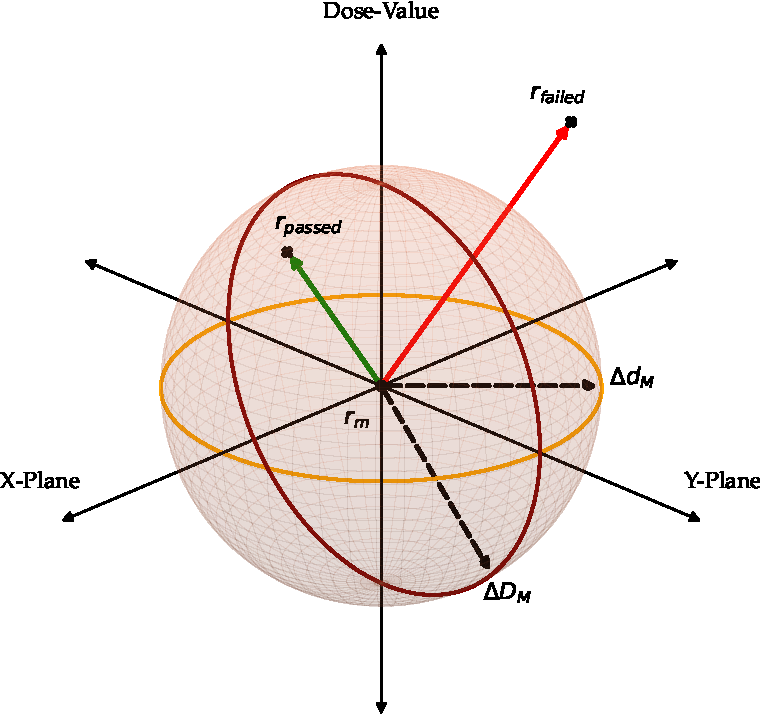
\includegraphics[width=0.5\textwidth]{gamma.pdf}
    \caption{Gamma test for two points $r_{passed}$ and $r_{failed}$ and the reference point $r_m$ for a 2D (X,Y) space. Orange and brown rings indicate distance and dose parameter acceptance margins respectively. The grey sphere represents the set of all points that pass the gamma test. Green and Red arrow indicate a passed and failed gamma test for the given reference point $r_m$, dose and spatial parameter.}\label{fig:gamma}
\end{figure}

\subsection{Hypotheses and Experiments}

In the following section we desribe several experiments which aim to investiage a certain hypothesis. All subsequent hypotheses are based on the previous listed hypothesis respectively and thus describe the developement process of the here proposed network. 

\subsubsection{General Applicability}\label{sssec:H1}
\begin{hanginglist}\itemsep2pt

    \item\textbf{Hypothesis 1}\newline
    The network is able to learn the general dose deposition process from the given input taken from a multitude of \acs{RT} segments of one tumor site. 
    Dose predictions for segments of the same entity are accurate and robust.\newpage

    \item\textbf{Experiment 1}\newline
    The proposed 3D-UNet was trained on a mutlitude of prostate cancer patient radio treatment segments. 
    Dose conformality was assessed with the gamma passrate for each individual test segment as well as entire test plans.\\

\end{hanginglist}

\subsubsection{Poor Initial Translatability}\label{sssec:H2}
\begin{hanginglist}\itemsep2pt

    \item\textbf{Hypothesis 2}\newline
    Different tumor sites vary drastically in segment shape, orientation and \ac{SSD}. The \acs{SSD} is, compared to other entities such as \acs{HN}, approximately constant for prostate cancer patients. The same holds true for tissue homogenity aspects of the respective body regions, when comparing lower abdomen to e.g. \acs{HN}. 
    Therefore, we hypothesize that the network will not achieve the gamma pass rates achieved so far nor sufficient ones when tested at different tumor sites and patient anatomies.\\

    \item\textbf{Experiment 2}\newline
    The from \emph{\ref{sssec:H1} \nameref{sssec:H1}} trained network was then used for inference on additional testing data from a multitude of tumor entities as well as patient anatomies to test its translational capabilities to a varying set of input characteristics.\\

\end{hanginglist}

\subsubsection{Increased Robustness}\label{sssec:H3}
\begin{hanginglist}\itemsep2pt

    \item\textbf{Hypothesis 3}\newline
    The inclusion of a broader variety of segment shapes, sizes and positions inside the patients anatomy, as well as differing body regions and therefore varying \acs{SSD} values and tissue densities results in a better robustness of the networks prediction accuracy.
    We hypothesize that significant increases in accuracy regarding newly included entities can be achieved while the accuracy for the previously present entities remains stable.\\

    \item\textbf{Experiment 3}\newline
    Network architecture as well as training procedure of the in \emph{\ref{sssec:H1} \nameref{sssec:H1}} trained network were kept, while adding data from liver, breast and \acs{HN} segments into the pool of training data. 
    The total amount of segments remained approximately constant and the ratio of treatment plans per entity was equal.
    The translational capabilities were then assessed by testing the newly trained network on the entities that were included in the training data as well as additional \ac{LN} test cases. 
    Significance of results was assessed using the Wilcoxon singed-rank test.
    With this test design we investigated if the network performance decreased on prostate data by including new tumor sites into the training data.
    Additionally we assessed its performance on seen as well as unseen treatment plan data.
    We used \acs{LN} plan data as the unseen test data because \acs{LN}s are present all over the human body, which makes this anatomies aswell as \acs{RT} plans of this tumor site especially heterogeneous. 
    Due to the small size of \acs{LN}s, segment fieldsize was especially small, which we assumed to be the biggest challenge for the network.\\

\end{hanginglist}

\subsubsection{Underlying Physics}\label{sssec:H4}
\begin{hanginglist}\itemsep2pt

    \item\textbf{Hypothesis 4}\newline
    We hypothesized that basic physical dependencies, such as accurate dose depth profiles, correct mapping of penumbra and impact of the distance squared law will be learned by the network from the inclusion of a multitude of \acs{SSD}, patient anatomies, segment shapes, angles and sizes into the training data.
    Therefore we assumed that the predictions of dose deposition in basic homegenous phantoms will be accurately predicted with the training on the given heterogeneous dataset.\\

    \item\textbf{Experiment 4}\newline
    Artificial phantoms are used to investigate the physical accuracy of the dose predictions of the networks from \emph{\ref{sssec:H1} \nameref{sssec:H1}} and \emph{\ref{sssec:H3} \nameref{sssec:H3}} at various positions. Phantoms consist of a water volume placed inside a $600~\times~600~\times~600~mm^3$ air volume at differing positions. With the default voxel dimensions of $1.1718~\times~1.1718~\times~3mm^3$ this results in a volume of shape $512~\times~512~\times~200~voxel$ for the phantom. 
    Water phantom dimensions will be $100 \times 512 \times 200~voxels$.
    Comparing dose cruves in the different spatial directions of a $10 \times 10 cm^2$ square field and 0° beam angle and the respective dose prediction yields information about the networks capability to learn the underlying physics.\\

\end{hanginglist}

\subsection{Patient Data}

All data used in the course of this study was taken from patients previously treated at the MR-Linac in our institution. 
All patients gave their informed written consent to this study, which was approved by the local ethical committee (ethics approval No. 659/2017BO1).
All treatment plans were created by a medical physicist in agreement with an oncologist. 
The training data consisted of two main datasets. 
One was used for the training of the in \emph{\ref{sssec:H1} \nameref{sssec:H1}} proposed network, which was only trained on prostate treatment data and consisted of 45 treatment plans with a total number of 2342 segments. 
The second dataset consisted of 15 treatment plans each for prostate, liver, breast and \acs{HN} tumor sites with 720, 819, 656 and 929 segments respectively. 
Additional 15 \acs{LN} cancer treatment plans with a total of 659 segments were used only for testing. 
A comprehensive summary of all training and testing data is given in \autoref{tab:patients} including training, validation, test split and information about the fieldsize distribution of training and test data. 


\begin{table}[htb]
\centering
    \scalebox{0.82}{
        \begin{tabular}{|lc|c|cccc|c|}
            \hline
                                                                                  &          & \multicolumn{1}{c|}{\textbf{Prostate}} & \multicolumn{4}{|c|}{\textbf{Mixed}}                                                      & \textbf{Testing} \\
            \textbf{}                                                             &          & \multicolumn{1}{c|}{\textit{}}         & \textit{Prostate} & \textit{Liver} & \textit{Mamma} & \multicolumn{1}{c|}{\textit{H\&N}} & \textit{LN}      \\ \hline
            \textbf{Patients}                                                     & \#       & 45                                     & 15                & 15             & 15             & 15                                 & 15               \\
            \textbf{Segments}                                                     & \#       & 2342                                   & 720               & 819            & 656            & 929                                & 659              \\
            \textbf{Split}                                                        & \#/\#/\# & 36/4/5                                 & 8/2/5             & 8/2/5          & 8/2/5          & 8/2/5                              & 0/0/15           \\
            \textbf{\begin{tabular}[c]{@{}l@{}}Fieldsize\\ Training\end{tabular}} & $cm^2$   & 36.5 (17.9)                            & 35.5 (18.0)       & 24.1 (18.4)    & 40.7 (28.5)    & 63.0 (50.5)                        & N/A              \\
            \textbf{\begin{tabular}[c]{@{}l@{}}Fieldsize\\ Testing\end{tabular}}  & $cm^2$   & 34.5 (15.8)                            & 34.6 (15.9)       & 22.8 (14.4)    & 40.6 (38.0)    & 68.9 (53.6)                        & 26.0 (25.6)      \\ \hline
            \end{tabular}
    }
    \caption{
        Patient data information for prostate only trained network and mixed entity trained network and test data set consisting of \acs{LN}. 
        Split is given for training~/~validation~/~testing. 
        Fieldsizes are given as mean (standard deviation).
    }\label{tab:patients}
\end{table}
